\setcounter{figure}{0}

\section{20th August 2023: Sense and sensibility}
\subsection*{Text: Song of solomon 2:8-3:5}
  \begin{quote}
    [8] The voice of my beloved!
        Behold, he comes,
    leaping over the mountains,
        bounding over the hills.
    [9] My beloved is like a gazelle
        or a young stag.
    Behold, there he stands
        behind our wall,
    gazing through the windows,
        looking through the lattice.
    [10] My beloved speaks and says to me:
    “Arise, my love, my beautiful one,
        and come away,
    [11] for behold, the winter is past;
        the rain is over and gone.
    [12] The flowers appear on the earth,
        the time of singing has come,
    and the voice of the turtledove
        is heard in our land.
    [13] The fig tree ripens its figs,
        and the vines are in blossom;
        they give forth fragrance.
    Arise, my love, my beautiful one,
        and come away.
    [14] O my dove, in the clefts of the rock,
        in the crannies of the cliff,
    let me see your face,
        let me hear your voice,
    for your voice is sweet,
        and your face is lovely.
    [15] Catch the foxes for us,
        the little foxes
    that spoil the vineyards,
        for our vineyards are in blossom.”


    [16] My beloved is mine, and I am his;
        he grazes among the lilies.
    [17] Until the day breathes
        and the shadows flee,
    turn, my beloved, be like a gazelle
        or a young stag on cleft mountains.


        [1] On my bed by night
    I sought him whom my soul loves;
        I sought him, but found him not.
    [2] I will rise now and go about the city,
        in the streets and in the squares;
    I will seek him whom my soul loves.
        I sought him, but found him not.
    [3] The watchmen found me
        as they went about in the city.
    “Have you seen him whom my soul loves?”
    [4] Scarcely had I passed them
        when I found him whom my soul loves.
    I held him, and would not let him go
        until I had brought him into my mother’s house,
        and into the chamber of her who conceived me.
    [5] I adjure you, O daughters of Jerusalem,
        by the gazelles or the does of the field,
    that you not stir up or awaken love
        until it pleases.
  \end{quote}
\subsection*{Notes}
\begin{itemize}
  \item{\KH{I have no idea what Ps Loli is talking about...}}
  % \item{Point 2}
  % \item{\begin{figure}[H]
  %   \centering
  %   % 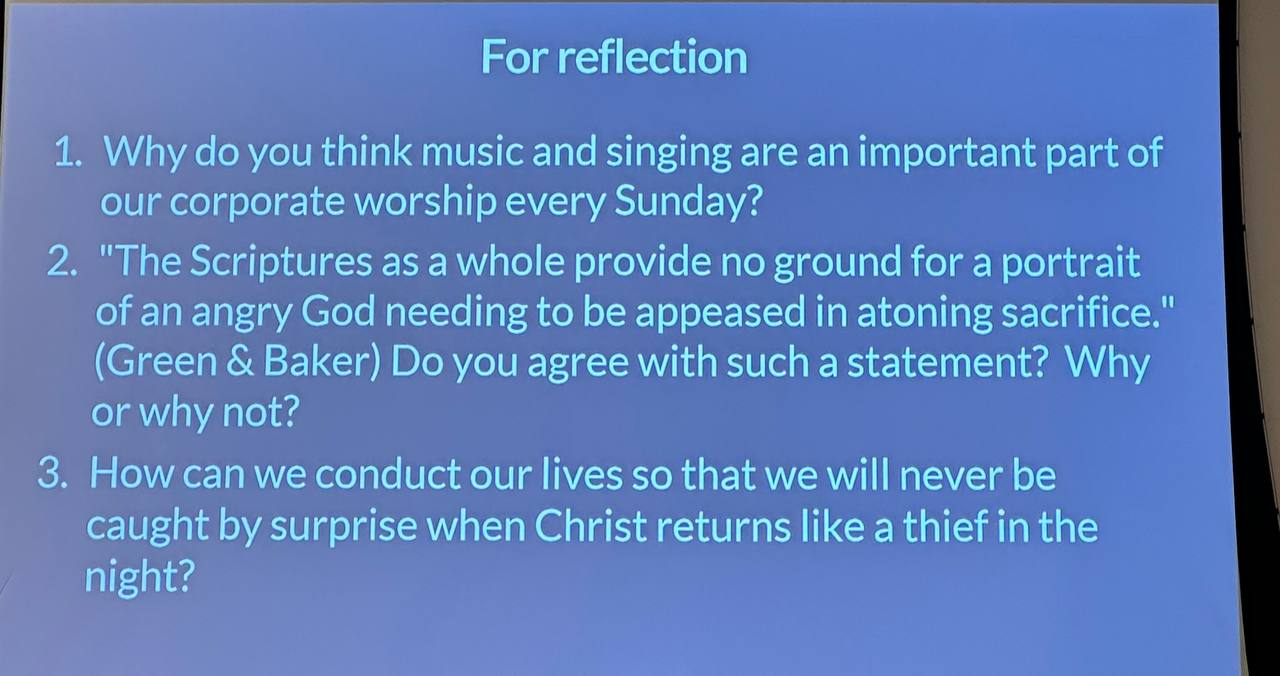
\includegraphics[width=0.8\textwidth, trim={0cm 0cm 0cm 0cm},clip]{Figures/marchSermon4Reflections.jpg}
  %   \includegraphics[width=0.8\textwidth, trim={0cm 0cm 0cm 0cm},clip]{example-image-a}
  %   \caption[]{Reflection questions for this sermon}
  %   \label{}
  % \end{figure}}
\end{itemize}